% This is samplepaper.tex, a sample chapter demonstrating the
% LLNCS macro package for Springer Computer Science proceedings;
% Version 2.20 of 2017/10/04
%
\documentclass[runningheads]{llncs}
%
\usepackage{graphicx}
\usepackage{amsmath}
\usepackage{cite}
\usepackage{hyperref}

% Used for displaying a sample figure. If possible, figure files should
% be included in EPS format.
%
% If you use the hyperref package, please uncomment the following line
% to display URLs in blue roman font according to Springer's eBook style:
 \renewcommand\UrlFont{\color{blue}\rmfamily}

\begin{document}
%
\title{Application of Machine Learning to Increase the Efficiency of the Global Search Algorithm for Solving Multicriterial Problems\thanks{This research was supported by the Russian Science Foundation, project No. 21-11-00204.}}
%
\titlerunning{Global Search Algorithm for Solving Multicriterial Problems}
% If the paper title is too long for the running head, you can set
% an abbreviated paper title here
%
\author{Konstantin Barkalov\orcidID{0000-0001-5273-2471} \and
Vladimir Grishagin\orcidID{0000-0002-2884-3670} \and
Evgeny Kozinov\orcidID{0000-0001-6776-0096}}
%
\authorrunning{K. Barkalov, V. Grishagin and E. Kozinov}
% First names are abbreviated in the running head.
% If there are more than two authors, 'et al.' is used.
%
\institute{Lobachevsky State University of Nizhni Novgorod, Nizhni Novgorod, Russia \email{\{konstantin.barkalov,evgeny.kozinov\}@itmm.unn.ru}, \email{vagris@unn.ru}}

%
\maketitle              % typeset the header of the contribution
%
	\begin{abstract}
Decision making models described as problems of multicriterial optimization are very complicated for investigation because the property of criteria contradictoriness leads to the notion of the solution as the set of non-dominated parameters (Pareto set). The complexity of these problems increases significantly in the case where criteria are multiextremal.
In the paper a novel algorithm for multicriterial black-box optimization with multiextremal criteria is considered. This algorithm applies ideas of complexity reduction when the initial multicriterial problem is reduced to a set of univariate scalar subproblems on the base of Peano mapping and maximum convolution. For solving univariate problems an information-statistical global optimization algorithm with guaranteed convergence to global optimum is used. As a core of novelty, this algorithm includes in its computational scheme a machine learning procedure with combination of accumulating the information of solved subproblems that allows one to significantly accelerate building the Pareto set.
Effectiveness of the proposed approach is estimated in the representative computational experiment on test sets of multicriterial problems with multiextremal criteria for different dimensions in comparison with several nature-inspired multiobjective optimization algorithms.


\keywords{Multicriterial problems \and Global optimization \and Logistic regression}
\end{abstract}
%
%
%
\section{Introduction}
Artificial intelligence models formulated as decision-making problems are extremely diverse and attract significant attention of researchers due to the richness of theoretical background and practical importance. The high complexity of decision-making models requires the development of new ideas that reduce this complexity. A promising way to improve decision-making algorithms is to combine in their development the advantages of different approaches. For example, machine learning procedures effectively use built-in optimization methods to enhance the quality of learning. 

In present paper we, on the contrary, propose an approach in which a machine learning technique embedded into optimization algorithm allows one to increase its efficiency when this algorithm is applied to solving complicated multiobjective problems. 

As the decision-making model we consider the multicriterial multidimensional optimization problems with multiextremal ``black-box'' criteria herein after called as MMCO problems. Combination of multicriteriality and multiextremality generates the dramatic complexity of these problems, because, first, criteria are contradictory, as a rule, and this circumstance leads to a complicated concept of solution (Pareto set) in such problems and, second, in the multiextremal case the growth of computational efforts is exponential when increasing the dimensionality (number of independent variables).

For analyzing multiobjective problems under consideration the following general approaches can be used. One of them is based on placement of a grid (deterministic or random) in the feasible domain, pairwise comparison of grid nodes in accordance with the domination principle and selection of non-dominated points. 

The second approach applies meta-heuristic methods (genetic algorithms, simulation annealing, particle swarm optimization, artificial bee or ant colony, firefly algorithm, etc.) inspired by modeling the behavior of biological agents \cite{Nebro2009,RC05,Mostaghim2007,Durillo2010} or physical processes \cite{DPA02,ZLT01}. Methods of this class are simple enough for implementation, but because of heuristic nature they do not guarantee convergence to global optimum in multiextremal case. 

The third approach is based on the reduction of multicriterial problem to a family of single-criterion (scalar) optimization subproblems by means of convolution method and solving these subproblems by efficient mathematical programming algorithms \cite{Collette2004,Marler2009,Marler2004,Pardalos2017,Wierzbicki,Ehrgott2005,GergelKozinov2020}. Under corresponding conditions, the solution of the scalar subproblem is a Pareto-optimal point. When changing coefficients of the convolution it is possible to find an approximation of the Pareto set. If the criteria in the initial multiobjective statement are multiextremal, the reduced convolution function is multiextremal as well, and for its optimization it is necessary to apply search algorithms that provide the finding of the global optimum. 

In the class of deterministic methods for multiextremal optimization with guaranteed convergence to global optimum \cite{Gablonsky2001,Sergeyev2010,Sergeyev2006,Evtushenko2014,Strongin2003,Sergeyev2013}, the algorithms developed in the framework of the information-statistical approach (ISA) \cite{Gergel2018,Barkalov2018} are among the most effective. The present paper describes a new algorithm belonging to the ISA class and aimed at solving MMCO problems that accelerates the Pareto set building by the application of machine learning ideas. 

The proposed method sequentially implements the concept of complexity reduction. Following this way, the initial MMCO problem is reduced to a family of single-criterion optimization subproblems by means of parameterized convolution. Then each multidimensional subproblem is transformed to an equivalent univariate (one-dimensional) optimization problem formed on the base of Peano-type mapping \cite{Evtushenko2014,Gergel2018,Marler2004,Pardalos2017}. Further, a special global optimization algorithm designed on the ISA platform is applied for solving the univariate problems. Its computational scheme includes two accelerators that decreases significantly number of algorithm's iterations. The first one when solving current one-dimensional problem takes into account results of iterations of all the previous problems solved already. The second mechanism influences the choice of the new iteration point estimating possible closeness of its pre-image in the criteria space to the Pareto set. This estimation is carried out by the method of separation planes, which is widely used in machine learning. 

For efficiency confirmation of the proposed approach combining the global optimization algorithm with machine learning procedures, the representative computational experiment has been conducted on the test class of multiextremal multicriterial problems of different dimensions. For expanding the confirmation area, the test problems were solved by several known meta-heuristic methods of multicriterial optimization. The Hyper-Volume (HV) index reflecting the quality of the Pareto set approximation was used as a comparison criterion. The results of the experiment have demonstrated significant advantages of the new algorithm over other methods having involved in comparison.

The rest of the paper is organized as follows. Section \ref{sec:2} contains statement of the problem to be considered. Section \ref{sec:3} is devoted to the description of the proposed algorithmic schemes.  Results of computational experiment are presented in Section \ref{sec:4}. Section \ref{sec:5} concludes the article.

\section{Problem statement}\label{sec:2}

The decision making model to be considered hereinafter as the MMCO problem can be described in the following statement.

Let real-valued functions $\varphi_s(y)$, $1 \leq s \leq k$, depend on vector of independent variables 
$y=(y_1, y_2, \dots, y_n)$ and are defined over a box-domain (hyperparallelepiped)
\begin{equation}
\label{eq:01}
    H=\{y \in R^n : a_i \leq y_i \leq b_i, 1 \leq i \leq n\}
\end{equation}                                      in $n$-dimensional Euclidean space $R^n$.

In decision making terminology the region (\ref{eq:01}) is called \textit{feasible domain}, the argument $y$ belonging to the domain (\ref{eq:01}) is \textit{feasible decision}.  Functions  $\varphi_s(y)$, $1 \leq s \leq k$, are called \textit{partial criteria} of the problem. These functions can be interpreted as goals of decision making and, for certainty, we will assume that the less the function value, the better the result of achieving this goal.

Partial criteria form a vector-function called \textit{vector criterion}
\begin{equation}
\label{eq:02}
    \Phi(y) = (\varphi_1(y), \varphi_2(y), \dots, \varphi_k(y))
\end{equation}
and problem of multicriterial optimization is formulated as the problem of minimizing the vector function (\ref{eq:02}) over the domain (\ref{eq:01}):

\begin{equation}
\label{eq:03}
    \Phi(y) \to \min, y \in H.
\end{equation}

Unfortunately, finding a decision   that provides the minimal values for all partial criteria simultaneously is possible only in exceptional cases because, as a rule, partial criteria are contradictory, when decreasing one criterion leads to increasing the other.

For defining the solution in this case, the known concept of domination is introduced to exclude obviously unsatisfactory decisions \cite{Pardalos2017,Marler2009}.
\begin{definition}
Let $y, z \in H$. Vector $y$ is said to dominate vector $z (y \succ z)$ if  
\begin{equation}
    \label{eq:04}
    \varphi_s(y) \leq \varphi_s(z), 1 \leq s \leq k
\end{equation}
and there exists a number $t$, $1 \leq t \leq k$, such that $\varphi_t(y) < \varphi_t(z)$.
\end{definition}

After that, the set of non-dominated (efficient, Pareto optimal) points is considered as the solution to the multicriterial problem. Let's reproduce the strict relevant definitions.
\begin{definition}
A decision vector $y^* \in H$ is a Pareto optimal point if in the domain $H$ there is no vector $z, z\neq y^*$ dominating $y^*$.
\end{definition}
\begin{definition}
The set of all Pareto optimal points (Pareto set $P$) is the Pareto optimal solution to the MMCO problem (\ref{eq:03}).
\end{definition}


There exist different approaches to searching for Pareto points, briefly discussed in Introduction. In our research we have applied the convolution approach when the multicriterial problem is reduced to a family of scalar (single-criterion) problems such that the solutions to these problems are Pareto optimal points.

The parameterized function
\begin{equation}
    \label{eq:05}
    V(\mu, y) = \max_{1 \leq s \leq k} \mu_s \varphi_s(y)
\end{equation}
is taken as the convolution (so called \textit{maximum convolution}) where parameters $\mu_s, 1 \leq s \leq k$, (\textit{weight coefficients}) are such that 
\begin{equation}
    \label{eq:06}
    \mu_s \geq 0, 1 \leq s \leq k, \sum_{s=1}^k \mu_s=1.
\end{equation}
Vector
\begin{equation}
    \label{eq:06a}
    \mu = (\mu_1, \dots, \mu_k) 
\end{equation}
under conditions (\ref{eq:06}) belongs to a $(k-1)$-dimensional convex polyhedron in the Euclidean space  $R^k$.

If in the domain $H$ all the criteria 
\begin{equation}
    \label{eq:07}
    \varphi_s(y) > 0, 1 \leq s \leq k,
\end{equation}
then global minimizer of the problem
\begin{equation}
    \label{eq:08}
    W(\mu, y) = V(\mu, y) + \alpha \sum_{s=1}^k \mu_s \varphi_s(y) \to \min, \; y \in H,
\end{equation}
is a Pareto point of the problem (\ref{eq:03}) ($\alpha$  is a sufficiently small parameter) \cite{Wierzbicki,Marler2004}.

If one or more partial criteria are not positive, this is not too restrictive, because it is possible to convert this problem to the statement satisfying conditions (\ref{eq:07}) with preserving the Pareto solution.

Theoretically, for constructing the complete Pareto set of a problem (\ref{eq:02}) it is sufficient to solve problems (\ref{eq:08}) with all possible weight coefficients (vectors $\mu$ from polyhedron (\ref{eq:06})). However, when numerical solving we can deal with a finite number of problems (\ref{eq:08}) and, therefore, obtain only an approximation of the Pareto set. In these circumstances, important aspects are choice of weight coefficient and evaluation of approximation quality.

In our research we took weight coefficients as nodes of a uniform grid in the polyhedron (\ref{eq:06}). For assessment of the quality of Pareto set approximation obtained after solving problems (\ref{eq:08}) with mentioned weights, the HyperVolume index (HV-index) \cite{Evtushenko2014,Gergel2018} was applied as a traditional criterion of the approximation accuracy.


\section{Global Search Algorithm for Solving MMCO Problems}\label{sec:3}

\subsection{Preliminary Information}

In the framework of our consideration, the partial criteria $\varphi_s(y)$, $1 \leq s \leq k$, are supposed to be ``black-box'' functions and to satisfy in the feasible domain (\ref{eq:01}) the Lipschitz condition
\begin{equation}
    \label{eq:09}
    |\varphi_s(y') - \varphi_s(y'')| \leq L_s \|y'-y''\|, \; y', y'' \in H, \; 1 \leq s \leq k,
\end{equation}
where constant values $L_s$, $1 \leq s \leq k$, (Lipschitz constants) are usually unknown. Notation $\| \cdot \|$ represents the Euclidean norm in $R^n$.  

In general case, the functions satisfying the Lipschitz condition are multiextremal, therefore, the convolution (\ref{eq:05}) will be multiextremal and Lipschitzian as well. It means that for solving the problem (\ref{eq:08}) it is required to apply methods of nonlinear programming which provide finding the global optimum. There are many global optimization algorithms designed under different assumptions about properties of objective function; relevant references can be found, for instance, in monographs \cite{Pardalos2017,Marler2009,Sergeyev2013}. Some of them are theoretically substantiated and guarantee the convergence to global solution; the others are empirical, for example, nature-inspired methods that do not ensure finding the global optimum. 

The information-statistical algorithms \cite{Gergel2018,Barkalov2018,Strongin2003}  as deterministic methods with guaranteed convergence are among the most effective for analyzing multiextremal optimization problems. For solving multidimensional problems, these algorithms apply two approaches based on ideas of dimensionality reduction. In the framework of one approach the multidimensional problem is reduced to a family of univariate problems connected recursively (scheme of nested optimization) \cite{Gergel2019_2}. The other approach \cite{Gergel2018,Sergeyev2013} exploits the known fact that $n$-dimensional box (1) and the closed interval $[0,1]$ of the real axis are equipotent sets and there exist unambiguous and continuous mappings of this interval onto the hyperparallelepiped (1) called \textit{Peano-type curves} or \textit{evolvents}.

Peano mappings can be applied to solving the optimization problems in the following way. Let there be a $n$-dimensional continuous function $g(y)$ defined in the domain (\ref{eq:01}) and $y(x)$ is a Peano-type curve. Then the continuity of $g(y)$ and $y(x)$ allows one to assert that
\begin{equation}
    \min_{y\in H} g(y) = \min_{x\in[0,1]} g(y(x)),
\end{equation}
i.e. instead of minimization of the multidimensional function $g(y)$ in the domain (\ref{eq:01}) one can solve the minimization problem for the one-dimensional function $g(y(x))$ over the interval $[0,1]$.

However, because of fundamental characteristics of the mapping $y(x)$ the reduced function $g(y(x))$ does not retain Lipschitz property in the case of Lipschitzian partial criteria from (\ref{eq:02}). In this situation the function $g(y(x))$ satisfies the H{\" o}lder condition 
\begin{equation}
    \label{eq:10}
    |g(y(x')) - g(y(x''))| \leq G \left|x'-x''\right|^{1/n}, \; x', x'' \in [0,1],
\end{equation}
where $G>0$ is H{\" o}lder constant. If the function $g(y)$ satisfies the Lipschitz property with a constant $L$ then the function $g(y(x))$ will satisfy the inequality (\ref{eq:10}) with $G=2L\sqrt{n+3}$ \cite{Strongin2003,Sergeyev2013}.

Before starting the general description of the proposed algorithm, let's introduce some designations. 

Let the set $M$ contain the finite number $m$ of different weight vectors (\ref{eq:06a}):
\begin{equation}
    \label{eq:11}
    M=(\mu^1, \dots, \mu^m),
\end{equation}
where
\begin{equation}
    \label{eq:12}
    \mu^i=(\mu^i_k, \dots, \mu^i_k), \; 1 \leq i \leq m.
\end{equation}

The set $M$ generates a family   of scalar problems 
\begin{equation}
    \label{eq:13}
    W(\mu^i, y)= V(\mu^i, y) + \alpha \sum^k_{s=1}\mu^i_s \varphi_s (y) \to \min, \; y \in H, 1 \leq i \leq m.
\end{equation}

Let's denote as $f^i(x)$ the univariate function obtained in accordance with Peano mapping $y(x)$ from the function $W(\mu^i, y)$, i.e.,
\begin{equation}
    \label{eq:14}
    f^i(x) = W(\mu^i, y(x)), \; 1 \leq i \leq m.
\end{equation}

Minimization of a separate function $f^i(x)$ over interval $[0,1]$ allows one to find partial solution(s) of the initial MMCO problem (\ref{eq:03}) and solving all the problems
\begin{equation}
    \label{eq:15}
    f^i(x) \to min, \; x \in [0,1], \; 1 \leq i \leq m,
\end{equation}
enables to construct an approximation of the Pareto set.

The following computational scheme is proposed for solving the problems of the family (\ref{eq:15}). In this scheme, all the problems (\ref{eq:15}) are solved sequentially and during minimization of current function $f^i(x), i > 1$, the results of preceding problems $f^j(x) \to \min, 1 \leq j \leq i - 1,$ completed already are taken into account.

Before proceeding to the detailed description of the scheme, we will make some preliminary comments. 

Hereinafter the term ``trial'' will denote the evaluation of the objective function $f^i(x)$ at a point $x^j \in [0,1]$ and obtaining the vector (trial result)
\begin{equation}
    \label{eq:15a}
    \Omega^i(x^j)=(z^{i,j}, \omega^j_1, \dots, \omega^j_k),
\end{equation}
where $z^{i, j}=f^i(x^j)$, and the quantities
\begin{equation}
    \label{eq:16}
    \omega^i_s=\varphi_s(y(x^j)), 1 \leq s \leq k,
\end{equation}
are values of corresponding partial criteria at the point $x^j$. If a vector $M$ of weight coefficients (\ref{eq:11}) corresponds to the function (\ref{eq:14}) then 
\begin{equation}
    \label{eq:17}
    z^{i, j} = \max_{1\leq s \leq k} \mu_s \omega^j_s + \alpha \sum^k_{s=1} \omega^j_s.
\end{equation}

It should be noted that if the value (\ref{eq:17}) has been already calculated and the vector $\Omega^i(x^j)$ has been stored, then evaluation of another function with its weight coefficient set $M'=(\mu'^1, \dots, \mu'^k)$ at the point $x^j$ does not require the recalculation the partial criteria (\ref{eq:02}) because the value $z^{l, j}$ can be easily computed according to (\ref{eq:17}).

For this goal, it is useful to organize a special matrix of a posteriori information which will store results of all conducted trials, for example, in the form
\begin{equation}
    \label{eq:18}
A^i_p =
\begin{pmatrix}
x^1 & x^2 & \dots & x^p \\
z^{i,1} & z^{i,2} & \dots & z^{i,p} \\
\omega_1^{i,1} & \omega_1^{i,2} & \dots & \omega_1^{i,p} \\
\dots & \dots & \dots & \dots \\
\omega_k^{i,1} & \omega_k^{i,2} & \dots & \omega_k^{i,p}
\end{pmatrix}
\end{equation}
after implementing $p$ trials at points $x^1, x^2, \dots, x^p$ when minimizing a function $f^i(x)$ from (\ref{eq:15}).

\subsection{General Computational Scheme}

Before starting the described algorithm to build a Pareto set approximation, the set (\ref{eq:11}) of weight coefficient vectors is supposed to be given. In the framework of the statement (\ref{eq:01})--(\ref{eq:03}) this set generates the family of $m$ multidimensional scalar problems (\ref{eq:13}) and corresponding to those the family of $m$ univariate problems (\ref{eq:15}). 

The general algorithm consists of $m$ stages. At the $i$-th stage, solving the problem (\ref{eq:15}) for the function $f^i(x)$  is carried out.

At the beginning of each stage initial trials are implemented in $q$ given points $x^1, x^2, \dots, x^q \in [0,1]$.

At the first stage when $f^i(x)=f^1(x)$, $q=2$ and $x^1=0, x^2=1$. These two trials generate results $\Omega^1(x^1), \Omega^1(x^2)$ from (\ref{eq:15a}) and initial information matrix $A^1_2$ from (\ref{eq:18}). 

In all the stages after the first one $(i>1)$, the trial coordinates obtained in all previous stages are taken as points of initial trials at current stage. As the matrix $A^{i-1}_q$ contains values of all partial criteria at these points it is easy to recalculate values $z^{i,1}, z^{i,2}, \dots, z^{i,p}$ of function $f^i(x)$ according to (\ref{eq:17}) and to build the updated matrix $A^i_q$.

Further computational procedure can be described in the following manner.

Let after completing $p \geq q$ trials at points $x^1, x^2, \dots, x^p$ the matrix $A^i_p$ has been obtained. For computing a new trial point $x^{p+1}$ it is necessary to implement operations in accordance with the following rules.

\textbf{Rule 1.} Points $x^j, 1 \leq j\leq p,$ are ordered in increasing order and renumbered by subscripts, i.e.,
\begin{equation}
    \label{eq:19}
    x_0 = 0 < x_1 < \dots < x_{p-2} < x_{p-1} = 1.
\end{equation}
The values $u_j = f^i(x_j), 1\leq j \leq p,$ are juxtaposed to the points $x_j, 1\leq j \leq p$.

\textbf{Rule 2.} Current estimation $\gamma$ of the H{\" o}lder constant  
\begin{equation}
    \label{eq:20}
\gamma=
\begin{cases}
  \begin{matrix}
     \gamma \Gamma, & \Gamma >0 \\
     1, & \Gamma = 0 
  \end{matrix}
\end{cases}
\end{equation}
is computed, where
\begin{equation}
    \label{eq:21}
\Gamma=
\max_{1 \leq j \leq p-1} {\frac{|u_j - u_{j-1}|}{\rho_j} },
\end{equation}
\begin{equation}
    \label{eq:22}
\rho_j = \sqrt[n]{x_j-x_{j-1}},
\end{equation}
and $r>1$ is a parameter of the method.

\textbf{Rule 3.} In the set of trial coordinates $x_j, 1 \leq j \leq p$, non-dominated points are selected according to the rule of Definition 2 and all such points are considered as points belonging to current approximation of the Pareto set. All columns of the information matrix $A^i_p$ are marked up with labels 0 or 1 where 1 corresponds to non-dominated points and 0 to dominated ones.

\textbf{Rule 4.} In the criteria space on the base of the marked up matrix $A^i_p$ a separating hyperplane $L_p$ is constructed applying logistic regression \cite{Yu2011} as efficient tool of machine learning.

\textbf{Rule 5.} For each point $x_j, 1 \leq j \leq p$, the distance $d_j$ of the vector $(\varphi_1(x_j), \dots, \varphi_k(x_j))$ to the separating plane $L_p$ is determined. This distance is considered to be negative if vector is placed above the plane and positive otherwise (see Fig. \ref{fig:1}).

\begin{figure}
\centering
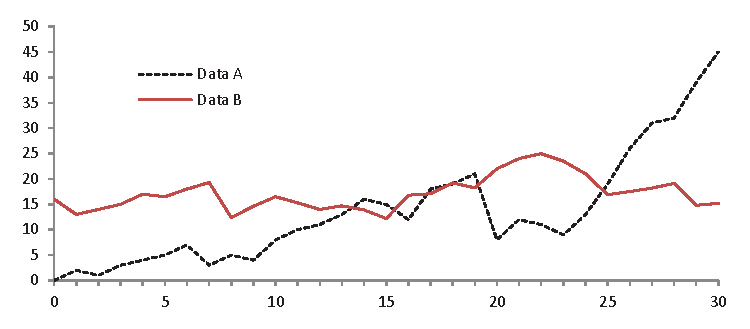
\includegraphics[width=0.5\textwidth]{fig1}
\caption{An example of estimating distances to the separating plane $L_p$.} \label{fig:1}
\end{figure}

\textbf{Rule 6.} Distances $d_j, 1 \leq j \leq p$, are scaled:     
\begin{equation}
    \label{eq:23}
d'_j=
\begin{cases}
  \begin{matrix}
     d_j / d_{max}, & d_j > 0 \\
     -d_j / d_{min}, & d_j < 0 
  \end{matrix}
\end{cases}
\end{equation}
where $d_{max} = \max_{1 \leq j \leq p} {d_j}$, $d_{min} = \min_{1 \leq j \leq p} {d_j}$.    

\textbf{Rule 7.} Neighboring points from (\ref{eq:19}) provide a partitioning of the interval $[0, 1]$ into $p-1$ subintervals $(x_{j-1}, x_j), 1 \leq j \leq p-1$.
A real value $B(j)$ is assigned to each subinterval $(x_{j-1}, x_j), 1 \leq j \leq p-1$. $B(j)$ is called \textit{the characteristic}  of this subinterval and is calculated as
\begin{equation}
    \label{eq:24}
    B(j) = \rho_j + \frac{(u_j-u_{j-1})^2}{\gamma^2 \rho_j} - \frac{2 (u_j+u_{j-1})}{\gamma} + \beta (d'_j + d'_{j-1}),
\end{equation}
where $\beta > 0$ is a parameter influencing the contribution of the separating plane. 

\textbf{Rule 8.} Among all subintervals, the subinterval $(x_{l-1}, x_l), 1 \leq l \leq p-1$, with the highest characteristic is chosen:
\begin{equation}
    \label{eq:25}
    B(l) = \max_{1 \leq j \leq p-1} {B(j)}.
\end{equation}

\textbf{Rule 9.} The new $(p+1)$-th trial is executed at the point  
\begin{equation}
    \label{eq:26}
    x^{p+1} = \frac{x_l + x_{l-1}}{2} - sign(u_l - u_{l-1}) \frac{1}{2r} \left(\frac{|u_l - u_{l-1}|}{\Gamma} \right)^n,
\end{equation}
values $\omega^{p+1}_s, 1 \leq s \leq k$, and $z^{i,p+1}=f^i(x^{p+1})$  are calculated and along with the point (\ref{eq:26}) they form the new matrix $A^i_{p+1}$ adding new column to the matrix $A^i_p$. 

\textbf{Rule 10.} If the inequality
\begin{equation}
    \label{eq:27}
    \rho_l=\sqrt[n]{x_l-x_{l-1}} < \varepsilon
\end{equation}
is true, where $\varepsilon > 0$ is predefined accuracy, then the $i$-th  stage (minimization of function $f^i(x)$) is over.

In the case $i < m$, the method proceeds to the next stage $(i = i+1)$.  

If $i=m$, then the algorithm completes its running and the set of non-dominated trial points in the criteria space is taken as a Pareto set approximation.

\section{Experimental efficiency testing}\label{sec:4}

Computations were conducted on the supercomputer ``Lobachevsky'' of the Nizhni Novgorod State University (operating system CentOS 7, control system SLURM). %One node of the supercomputer has 2 processors Intel Sandy Bridge E5-2660 2.2 GHz, 64 Gb RAM. One CPU contains 8 cores, i.e., 16 cores are available on one node. 
To obtain the executable program code the compilers Intel C++ 17.0.0 and python 3.9 were used. Computations were performed with the support of the package scikit-learn 0.24.2 and the optimization software Globalizer \cite{globalizerSystem}.

The experiment was organized in the following way. For efficiency evaluation of the proposed algorithm hereinafter called AGS-SP (Algorithm of Global Search with Separating Planes), it was compared with its modification AGS-R (Algorithm of Global Search Reduced) where computational scheme is similar, but Rules 3 -- 6 are removed and in the characteristic (\ref{eq:24}) parameter $\beta = 0$. AGS-R ignores the information about the Pareto set approximation. Moreover, to expand the basis of the comparison, some known meta-heuristic evolutionary MMCO methods were involved into the experiment, namely, algorithms SMPSO \cite{NDG09}, OMOPSO \cite{RC05}, NSGA-II \cite{DPA02}, SPEA2 \cite{ZLT01}, IBEA \cite{ZK04} from the jMetal framework \cite{DNA10}.

As a criterion of effectiveness, the HyperVolume (HV) index \cite{Evtushenko2014,Gergel2018} were adopted. It is traditionally used to estimate the efficiency of the quality for Pareto set approximations built by numerical methods. HV-index characterizes the completeness of the approximation (a larger value corresponds to a more complete coverage of the Pareto region). To compare correctly the relative effectiveness of different methods in a unified scale the ``ideal'' value of HV index was calculated on a dense grid in the feasible domain for each test MMCO problem

Three series of experiments were executed. The first one dealt with a simple problem and was aimed at demonstration of positive influence of criteria space analysis by means of separating planes and at comparing with evolutionary techniques.
This problem was bi-criteria one \cite{CHIANDUSSI2012912}:
\begin{equation}
    \label{eq:28}
    \begin{matrix}
f_1 (y)=y_1, \\
f_2 (y)=(1+10y_2 )[1- \left(\frac{y_1}{1+10y_2} \right)^2- \frac{y_1}{1+10y_2} \sin(8 \pi y_1 ) ], \\
0 \leq y_1,y_2 \leq 1.
    \end{matrix}
\end{equation}

AGS-SP and AGS-R solved 20 scalar problems (\ref{eq:08}) for different weight coefficients $\mu_1$ uniformly distributed in the interval $[0,1]$ (the second weight coefficient $\mu_2=1-\mu_1$ due to (\ref{eq:06})). Both the methods used the same parameters $r=2$ and $\varepsilon=0.01$ and the parameter $\beta=0.01$ was taken in AGS-SP. Each evolutionary method was launched 100 times and the HV index was averaged.
Results of the first experiment are presented in Table \ref{tab:01}.

\begin{table}[ht]
\caption{Results of solving the MMCO problem (\ref{eq:28}).}
\label{tab:01}
\center
\begin{tabular}{|c|c|c|c|}
\hline
\textbf{Algorithm} & \textbf{Number of trials} & \textbf{Number of Pareto points} & \textbf{HV}    \\ \hline
Pareto HV          & ---                       & ---                              & \textbf{1.202} \\
AGS-R              & 300                       & 33                               & \textbf{1.146} \\
AGS-SP             & 226                       & 34                               & \textbf{1.146} \\
SMPSO              & 300                       & 15.75                            & 1.072          \\
OMOPSO             & 300                       & 15.89                            & 1.136          \\
NSGAII             & 300                       & 37.62                            & 0.913          \\
SPEA2              & 300                       & 38.32                            & 0.894          \\
IBEA               & 300                       & 41.99                            & 0.985          \\ \hline
\end{tabular}
\end{table}

The data of the table show that AGS-SP and AGS-R solve the problem (\ref{eq:28}) more efficient than evolutionary methods because while spending the same number of trials (and even less as AGS-SP) they provide the  better HV index and find more points in Pareto set approximation. If to compare AGS-SP and AGS-R with each other, then AGS-SP has an advantage due to HV indices being the same, but AGS-SP was ``faster'' as it executed fewer trials.

The second series was aimed to studying the influence of the parameter $\beta$ from (\ref{eq:24}) on number of trials produced by AGS-SP and HV index. Bi-criteria problems were considered where complicated multiextremal two-dimensional random functions \cite{Grishagin2015_2} were taken as partial criteria. The level curves of some of them are shown in Fig.  \ref{fig:2}. 50 MMCO problems of this type have been solved with the same parameters $r=3, \varepsilon=0.01$ and number $m=50$ of weight coefficient vectors (\ref{eq:11}) for different values of the parameter $\beta$ from the interval $[0,0.1]$. After solving 50 MMCO problems the results were averaged for each separate $\beta$. The change of HV and the number of trials depending on $\beta$ is shown in Fig. \ref{fig:3}.

As it can be seen, the growth of the parameter $\beta$ leads to significant decrease in the number of trials. At the same time, when increasing $\beta$, the value of the HV index deteriorates. As it follows from the graphs, the value $\beta=0.01$ can be taken as a good enough compromise.

\begin{figure}
\centering
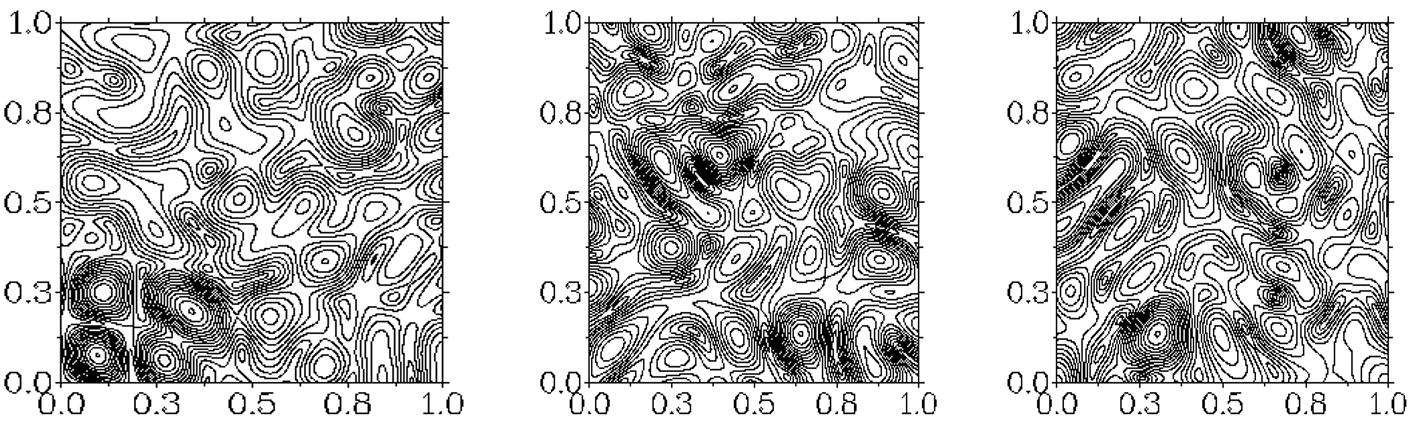
\includegraphics[width=\textwidth]{fig2}
\caption{The level curves for test function.} \label{fig:2}
\end{figure}

\begin{figure}
\centering
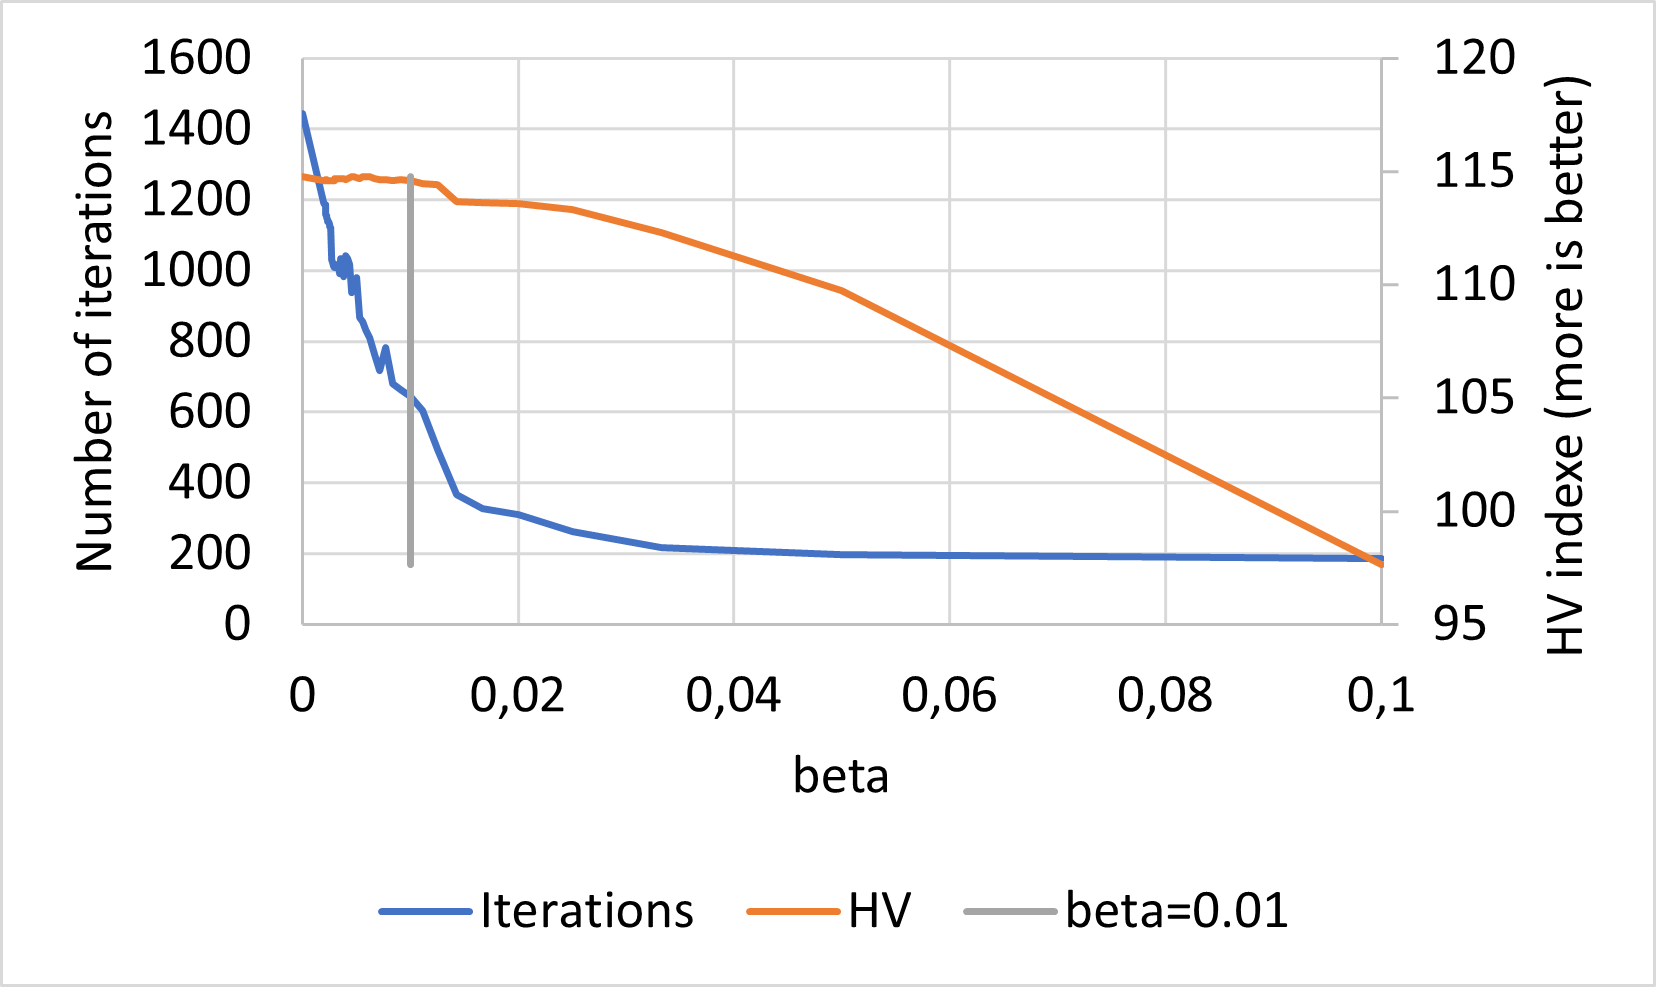
\includegraphics[width=0.7\textwidth]{fig3}
\caption{Influence of the parameter $\beta$.} \label{fig:3}
\end{figure}

Problems with greater dimension were solved in the third series of experiments. Multiextremal functions of the class GKLS \cite{Gaviano2003} have been chosen as partial criteria of the MMCO problems.  In global optimization this class is widely used for testing global search algorithms. Bi-criteria problems of dimensions $n=3$ and $n=4$ were considered. Weight coefficients were chosen as nodes of a uniform grid in the domain defined by the conditions (\ref{eq:06}) with number of nodes equal to 200 in 3-dimensional case and to 50 for $n=4$. 100 MMCO problems were participated in the experiment for each dimension. AGS-R and AGS-SP used the same parameter $r=4.5$. AGS-SP applied the parameter $\beta=0.05$ for the dimension $n=3$ and $\beta=0.025$ in the case of $n=4$.  Running of each evolutionary method was repeated 10 times and results were averaged.   

All the competing methods solved the set of 100 MMCO problems several times such that in each case they executed different number of trials and, correspondingly, obtained different values of HV's. If we take a method, consider all the pairs $(K, HV(K))$ where $K$ is number of trials executed by the method and $HV(K)$ is the corresponding value of the HV-index, and place all these pairs as points on the plane with coordinate abscissa axis $K$ and ordinate axis $HV$ we build so called \textit{operational characteristic} \cite{Grishagin2016_2} of the method. On the base of operational characteristics it is easy to compare visually the efficiency of different methods. Indeed, if the operational characteristic of one method is located above the characteristic of the other, then the first method is better because it spends fewer trials for obtaining the same HV, or, equivalently, the first method provides better HV for the same number of trials. Operational characteristics of the competing algorithms for dimensions 3 and 4 are presented in Fig. \ref{fig:4} and \ref{fig:5} correspondingly.
 
\begin{figure}
\centering
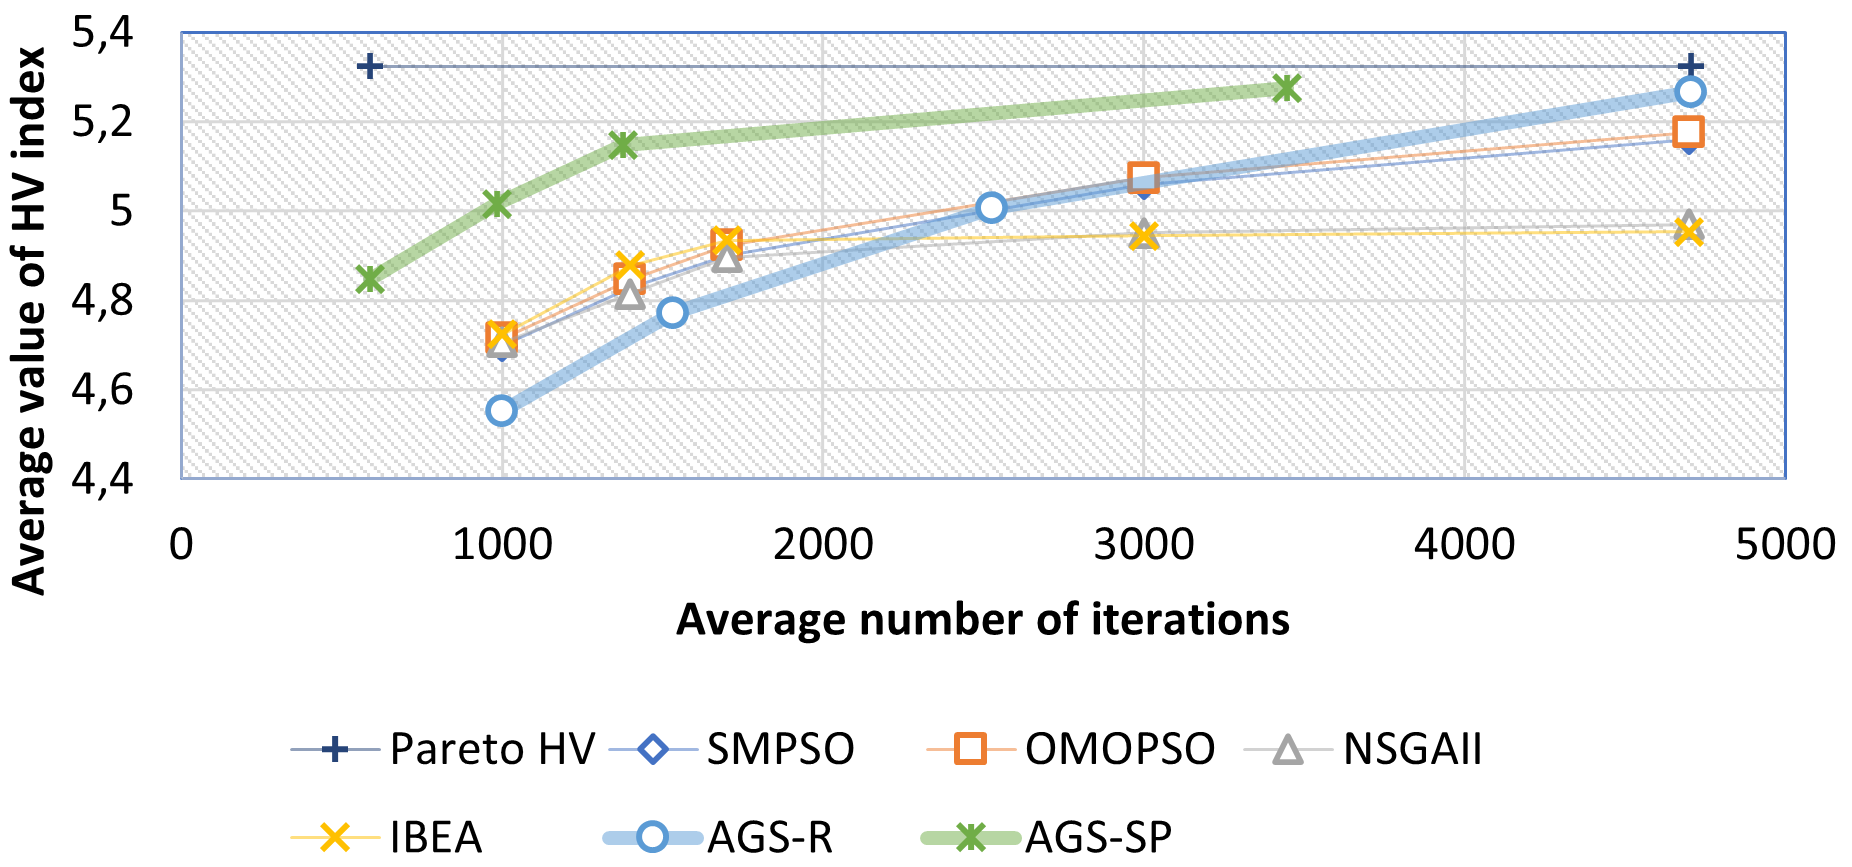
\includegraphics[width=0.9\textwidth]{fig4}
\caption{Operational characteristics for dimension 3.} \label{fig:4}
\end{figure}

\begin{figure}
\centering
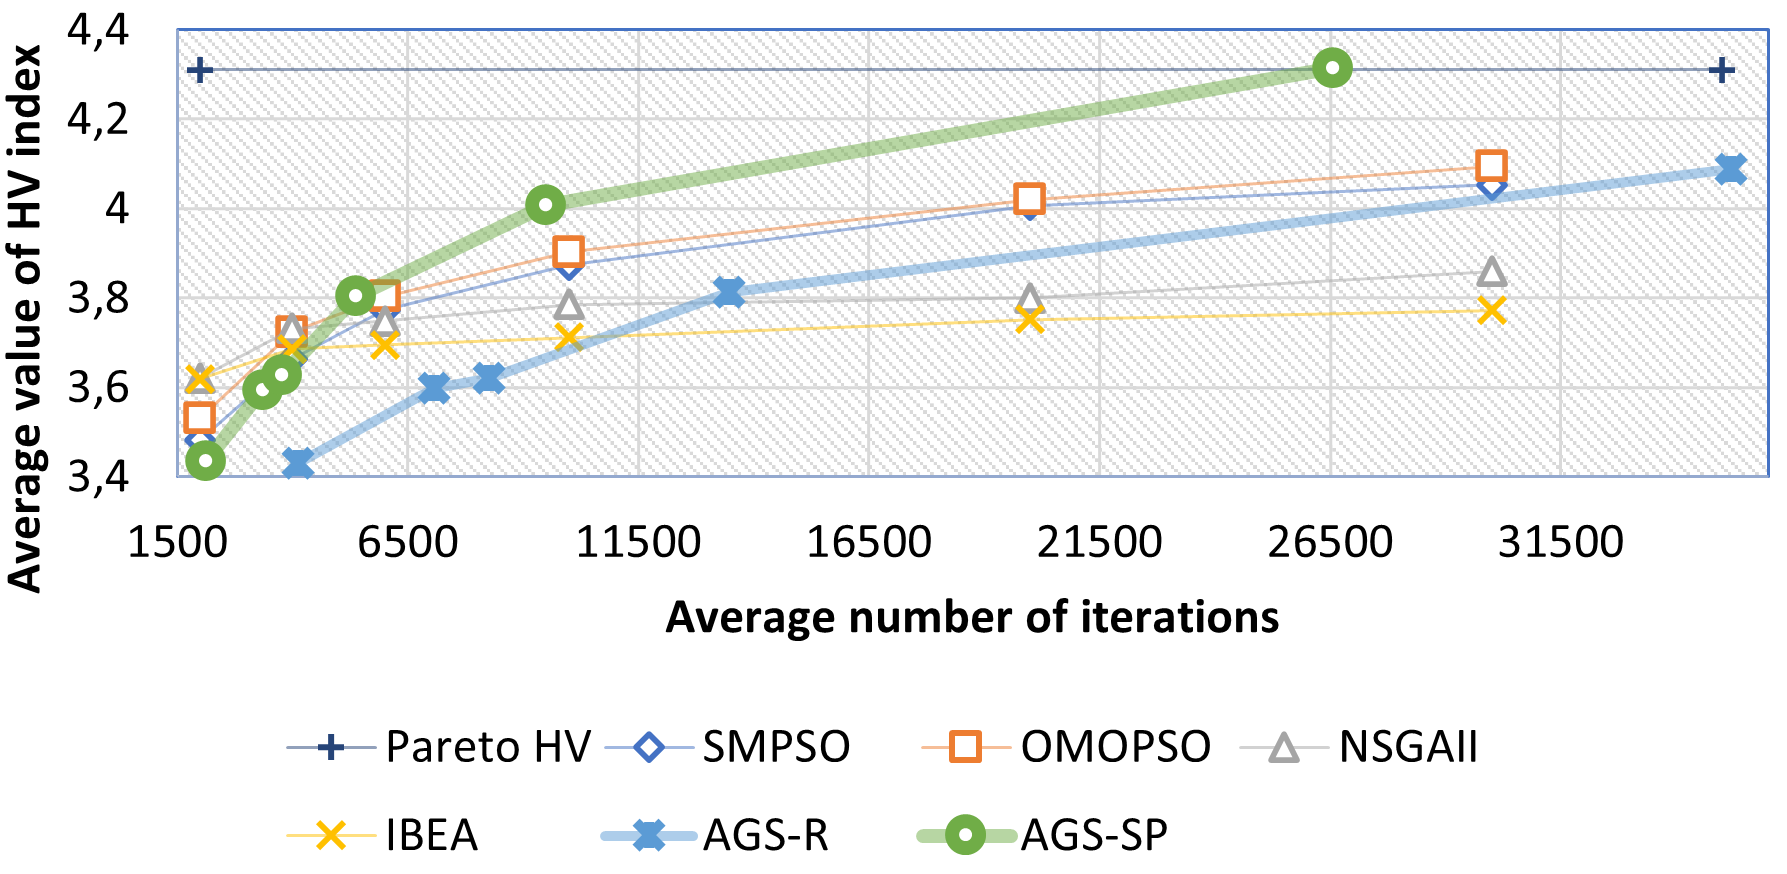
\includegraphics[width=0.9\textwidth]{fig5}
\caption{Operational characteristics for dimension 4.} \label{fig:5}
\end{figure}

As it follows from the results for the multidimensional cases, the undisputed winner is the proposed algorithm AGS-SP, i.e., the applied modifications enhance significantly the efficiency of solving complicated multiextremal multicriterial problems and allow obtaining better approximation of the Pareto set. And what's more, AGS-SP achieves the best possible value of HV-index in the 4-dimensional experiment while the other methods are far from the best level.


\section{Conclusion}\label{sec:5}

In the paper a new numerical method for solving multidimensional multicriterial  optimization problems has been proposed for the case of multiextremal black-box partial criteria. The novelty of the method consists in application of logistic regression as a tool, widely used in machine learning, for planning iterations of the global optimization algorithm. The workability and efficiency of the method have been evaluated in a representative experiment on test classes of multiextremal problems of different dimensions. In the experiment the proposed method was compared to its version which does not utilize logistic regression and to several known evolutionary methods. All the experiments have demonstrated significant advantages of the new method over other competitors.

The further development of the research will be associated with designing parallel generalizations of the method exploiting ideas of parallel characteristical algorithms and oriented at high-performance  supercomputers.


%
% ---- Bibliography ----
%
% BibTeX users should specify bibliography style 'splncs04'.
% References will then be sorted and formatted in the correct style.
%
% \bibliographystyle{splncs04}
% \bibliography{mybibliography}
%
\bibliographystyle{splncs04}
\bibliography{bibliography}


% \begin{thebibliography}{8}
% \bibitem{ref_article1}
% Author, F.: Article title. Journal \textbf{2}(5), 99--110 (2016)

% \bibitem{ref_lncs1}
% Author, F., Author, S.: Title of a proceedings paper. In: Editor,
% F., Editor, S. (eds.) CONFERENCE 2016, LNCS, vol. 9999, pp. 1--13.
% Springer, Heidelberg (2016). \doi{10.10007/1234567890}

% \bibitem{ref_book1}
% Author, F., Author, S., Author, T.: Book title. 2nd edn. Publisher,
% Location (1999)

% \bibitem{ref_proc1}
% Author, A.-B.: Contribution title. In: 9th International Proceedings
% on Proceedings, pp. 1--2. Publisher, Location (2010)

% \bibitem{ref_url1}
% LNCS Homepage, \url{http://www.springer.com/lncs}. Last accessed 4
% Oct 2017
% \end{thebibliography}
\end{document}
